\section{Sử dụng GraphRAG cho trả lời câu hỏi lịch sử}
\label{sec:graphrag}

\subsection{Kiến trúc tổng quan của GraphRAG}
\textbf{Trích xuất và Liên kết Thực thể:} Bước đầu tiên để hiểu câu hỏi trong ngữ cảnh của KG. Hệ thống sử dụng kết hợp nhiều phương pháp, từ khớp từ khóa và biểu thức chính quy cho các thực thể lịch sử thông dụng, đến các mô hình ngôn ngữ cho các trường hợp phức tạp hơn. Các thực thể được trích xuất sau đó trải qua quá trình Entity Linking để ánh xạ chính xác tới các nút chuẩn trong KG, xử lý các vấn đề coreference và alias thường gặp trong văn bản lịch sử.

\textbf{Hybrid Retrieval:} Đây là cốt lõi của hệ thống, sử dụng đa tín hiệu để cân bằng giữa recall và precision. Hệ thống kết hợp bốn nguồn tín hiệu chính: (1) điểm số từ kết quả liên kết thực thể, (2) tìm kiếm vector dựa trên độ tương đồng ngữ nghĩa, (3) full-text search với từ khóa, và (4) duyệt đồ thị để lấy ngữ cảnh từ các mối quan hệ của thực thể trong KG. Các ứng viên từ các nguồn này được tổng hợp, re-ranking và lựa chọn để tạo thành tập ngữ cảnh tối ưu.

\textbf{Context Builder \& Answer Generator:} Các đoạn văn bản được truy xuất được ghép nối trong giới hạn token của mô hình, đồng thời được bổ sung thông tin quan hệ từ KG để làm giàu ngữ cảnh. Dựa trên ngữ cảnh này và câu hỏi, một prompt chuyên biệt được xây dựng cho từng loại câu hỏi và đưa vào LLM để sinh câu trả lời cuối cùng. Toàn bộ quy trình được hỗ trợ bởi cơ chế bộ nhớ đệm và tối ưu hóa để đảm bảo hiệu năng thực thi.

\subsection{Query processing pipeline}

Quy trình xử lý một câu hỏi trong hệ thống GraphRAG diễn ra tuần tự qua một pipeline được tự động hóa, từ khi tiếp nhận câu hỏi thô đến khi đưa ra câu trả lời được kiểm chứng. Các bước chính được mô tả như sau:

\begin{enumerate}
    \item \textbf{Classification \& Preprocessing:} Hệ thống đầu tiên xác định loại câu hỏi là MCQ hoặc TF. Câu hỏi sau đó được chuẩn hóa. Đối với câu hỏi Đúng/Sai có kèm tư liệu, nội dung tư liệu được tách riêng để xử lý đặc biệt.

    \item \textbf{Extract và Liên kết Thực thể:} Các thực thể lịch sử được nhận diện trong câu hỏi và các lựa chọn (nếu có). Các thực thể này sau đó được ánh xạ tới các nút tương ứng trong KG thông qua cơ chế liên kết sử dụng kết hợp so khớp bề mặt và độ tương đồng ngữ nghĩa.

    \item \textbf{Hybrid Retriever và Re-ranker:} Từ các thực thể đã liên kết, hệ thống đồng thời khởi chạy nhiều chiến lược truy xuất: tìm kiếm vector ngữ nghĩa, tìm kiếm toàn văn với từ khóa, và duyệt đồ thị để thu thập các đoạn văn bản và quan hệ liên quan. Các ứng viên từ mọi nguồn được tổng hợp, xếp hạng lại bằng một mô hình re-ranker để đánh giá độ liên quan sâu, và cuối cùng được lựa chọn để tạo thành một tập ngữ cảnh gọn gàng, giàu thông tin.

    \item \textbf{Answer Generator:} Ngữ cảnh đã được truy xuất và làm giàu được đóng gói cùng với câu hỏi gốc vào một prompt được thiết kế chuẩn. Prompt này được đưa đến LLM, lúc này đóng vai trò là bộ tổng hợp và suy luận, để sinh ra câu trả lời văn bản. Câu trả lời thô sau đó được chuẩn hóa trích xuất ký tự 'A', 'B', 'C', 'D' với MCQ hoặc từ khóa "Đúng"/"Sai" với TF để so khớp với đáp án.

    \item \textbf{Post-processing \& Trust score:} Hệ thống có thể tính toán một điểm tin cậy (trust score) cho câu trả lời, dựa trên các yếu tố như chất lượng và sự phù hợp của ngữ cảnh được truy xuất, đồng thời ghi nhận lại các đoạn văn bản nguồn đã sử dụng để hỗ trợ cho khả năng giải thích và truy xuất nguồn gốc.
\end{enumerate}

\subsection{Tích hợp và Tối ưu hóa Hệ thống với Neo4j}

Cơ sở dữ liệu đồ thị Neo4j đóng vai trò là xương sống lưu trữ và truy vấn cho Knowledge Graph trong hệ thống. Sự tích hợp này mang lại những lợi thế đặc thù:

\begin{itemize}
    \item \textbf{Truy vấn Đồ thị Linh hoạt:} Neo4j cho phép thực thi hiệu quả các truy vấn Cypher phức tạp, như tìm kiếm đường đi ngắn nhất giữa các thực thể hoặc thu thập tất cả các mối quan hệ trong bán kính \(k\) bước từ một nút gốc. Điều này là then chốt để thực hiện suy luận đa bước (multi-hop reasoning).

    \item \textbf{Truy xuất Thông tin Hỗn hợp:} Ngoài truy vấn cấu trúc, Neo4j hỗ trợ tích hợp tìm kiếm toàn văn (full-text search) trên các thuộc tính văn bản của node và tìm kiếm vector (vector similarity search) trên embedding của chúng. Điều này cho phép thực hiện "truy xuất lai" ngay trong cùng một hệ thống cơ sở dữ liệu.

    \item \textbf{Quản lý Siêu dữ liệu và Truy xuất Nguồn gốc:} Mỗi quan hệ và thực thể trong đồ thị có thể được gắn kèm siêu dữ liệu (metadata) như nguồn tài liệu gốc, độ tin cậy của việc trích xuất. Khi truy vấn, thông tin này được trả về một cách tự nhiên, hỗ trợ mạnh mẽ cho việc truy xuất nguồn gốc (provenance) của câu trả lời.

    \item \textbf{Tối ưu hóa Hiệu năng:} Để đảm bảo thời gian phản hồi nhanh cho các truy vấn tương tác, hệ thống triển khai các cơ chế như bộ nhớ đệm có thời gian sống (TTL cache) cho kết quả truy vấn đồ thị và xử lý hàng loạt (batch processing) cho các thao tác đọc/ghi. Các chiến lược backoff cũng được áp dụng để xử lý lỗi tạm thời một cách tao nhã.
\end{itemize}

Kiến trúc kết hợp giữa sức mạnh biểu diễn ngôn ngữ của LLM và khả năng biểu diễn tri thức có quan hệ của Neo4j tạo nên một hệ thống hỏi đáp mạnh mẽ, đặc biệt phù hợp cho lĩnh vực lịch sử - nơi mà các mối liên hệ nhân quả, dòng thời gian và bối cảnh đóng vai trò trung tâm.

\begin{figure}[H]
\centering
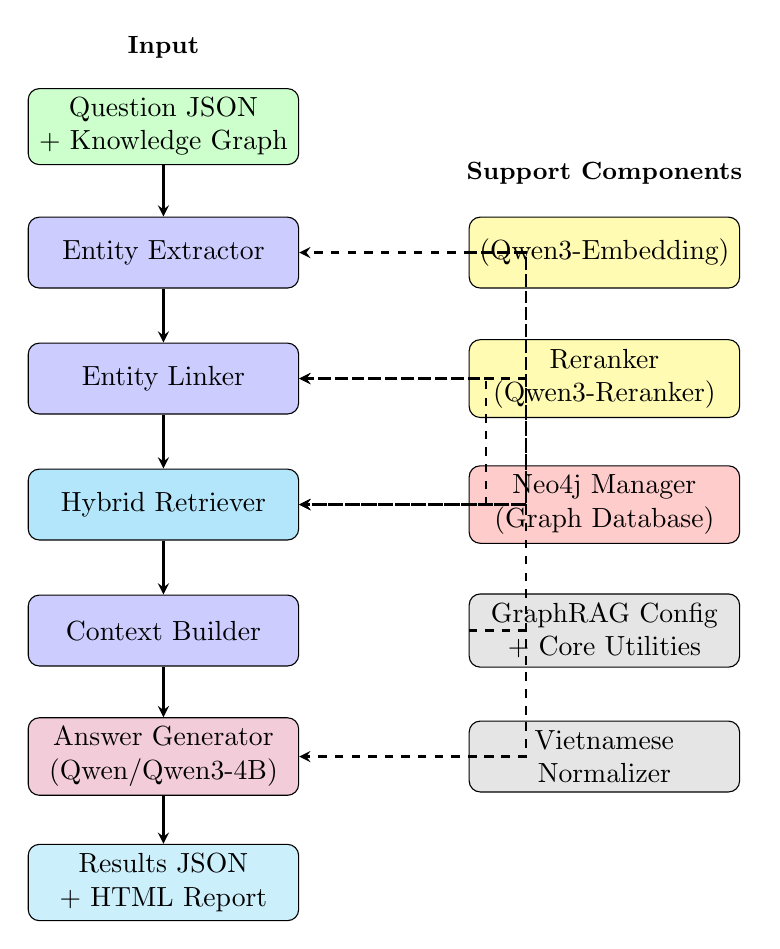
\begin{tikzpicture}[node distance=1.6cm, auto]
    % Styles
    \tikzstyle{datablock} = [rectangle, draw, fill=green!20, 
        text width=3.2cm, text centered, rounded corners, minimum height=0.9cm]
    \tikzstyle{component} = [rectangle, draw, fill=blue!20, 
        text width=3.2cm, text centered, rounded corners, minimum height=0.9cm]
    \tikzstyle{apiblock} = [rectangle, draw, fill=orange!20, 
        text width=3.2cm, text centered, rounded corners, minimum height=0.9cm]
    \tikzstyle{dbblock} = [rectangle, draw, fill=red!20, 
        text width=3.2cm, text centered, rounded corners, minimum height=0.9cm]
    \tikzstyle{modelblock} = [rectangle, draw, fill=purple!20, 
        text width=3.2cm, text centered, rounded corners, minimum height=0.9cm]
    \tikzstyle{outputblock} = [rectangle, draw, fill=cyan!20, 
        text width=3.2cm, text centered, rounded corners, minimum height=0.9cm]
    \tikzstyle{arrow} = [thick,->,>=stealth]
    \tikzstyle{dashedarrow} = [thick,->,>=stealth,dashed]
    
    % === LEFT COLUMN: Main Pipeline ===
    \node [datablock] (input) {Question JSON\\+ Knowledge Graph};
    \node [component, below of=input] (entityext) {Entity Extractor};
    \node [component, below of=entityext] (entitylink) {Entity Linker};
    \node [component, below of=entitylink, fill=cyan!30] (retriever) {Hybrid Retriever};
    \node [component, below of=retriever] (ctxbuilder) {Context Builder};
    \node [modelblock, below of=ctxbuilder] (answergen) {Answer Generator\\(Qwen/Qwen3-4B)};
    \node [outputblock, below of=answergen] (output) {Results JSON\\+ HTML Report};
    
    % === RIGHT COLUMN: Components ===
    \node [component, right of=entityext, xshift=4cm, fill=yellow!30] (embedding) {(Qwen3-Embedding)};
    \node [component, below of=embedding, fill=yellow!30] (reranker) {Reranker\\(Qwen3-Reranker)};
    \node [dbblock, below of=reranker] (neo4j) {Neo4j Manager\\(Graph Database)};
    \node [datablock, below of=neo4j, fill=gray!20] (config) {GraphRAG Config\\+ Core Utilities};
    \node [datablock, below of=config, fill=gray!20] (normalizer) {Vietnamese\\Normalizer};
    
    % === ARROWS: Main Flow ===
    \draw [arrow] (input) -- (entityext);
    \draw [arrow] (entityext) -- (entitylink);
    \draw [arrow] (entitylink) -- (retriever);
    \draw [arrow] (retriever) -- (ctxbuilder);
    \draw [arrow] (ctxbuilder) -- (answergen);
    \draw [arrow] (answergen) -- (output);
    
    % === ARROWS: Dependencies (Phương pháp 1) ===
    \draw [dashedarrow] (embedding) -- ++(-1,0) |- (entitylink);
    \draw [dashedarrow] (embedding) -- ++(-1,0) |- (retriever);
    \draw [dashedarrow] (reranker) -- ++(-1,0) |- (retriever);
    \draw [dashedarrow] (neo4j) -- ++(-1.5,0) |- (entitylink);
    \draw [dashedarrow] (neo4j) -- ++(-1.5,0) |- (retriever);
    \draw [dashedarrow] (config) -- ++(-1,0) |- (answergen);
    \draw [dashedarrow] (normalizer) -- ++(-1,0) |- (entityext);
    
    % === Labels ===
    \node [above of=input, yshift=-0.6cm, font=\small\bfseries] {Input};
    \node [above of=embedding, yshift=-0.6cm, font=\small\bfseries] {Support Components};
\end{tikzpicture}
\caption{Kiến trúc tổng quan của GraphRAG}
\label{fig:method1}
\end{figure}